
\PassOptionsToPackage{unicode}{hyperref}
\PassOptionsToPackage{naturalnames}{hyperref}
\documentclass{beamer} 
%\usepackage{babel}
%\usepackage[utf8]{inputenc}


%%% FONT SELECTION %%%%%%%%%%%%%%%%%
%%% we choose a sans font %%%%%%%%%%
\usepackage{kmath,kerkis} 
%\usepackage[default]{gfsneohellenic} 
%%%%%%%%%%%%%%%%%%%%%%%%%%%%%%%%%%%%

\usepackage{color}
\usepackage{amsmath}
\usepackage{amssymb}

\usepackage{epstopdf}
\usepackage{graphicx}
\graphicspath{{./images/presentation}}

%%
% load TEI-Pel - specific layout
\usepackage{TeiPel_En_Beamer_Layout}
\setTeipelLayout{draft,newlogo}% options: "draft", "newlogo"



% Thesis Info - first page 
	% title
		\title[Gravimetric Sensing Aided by Radiation Cooling]{Gravimetric Sensing Aided by Radiation Cooling}		
    %\author
		\author[Yishai Arieli]{Yishai Arieli}
	% supervisor	
		\supervisor{Supervisor}{Professor Howell}
	% date
		\presentationDate{October 22, 2021}


\begin{document}

% typeset front slides
	\typesetFrontSlides

% Your Slides Start here:
\section{Theoretical background}
\subsection{Torsional pendulum}
% frame 1
\begin{frame}{Harmonic oscillator}
	\begin{center}		
		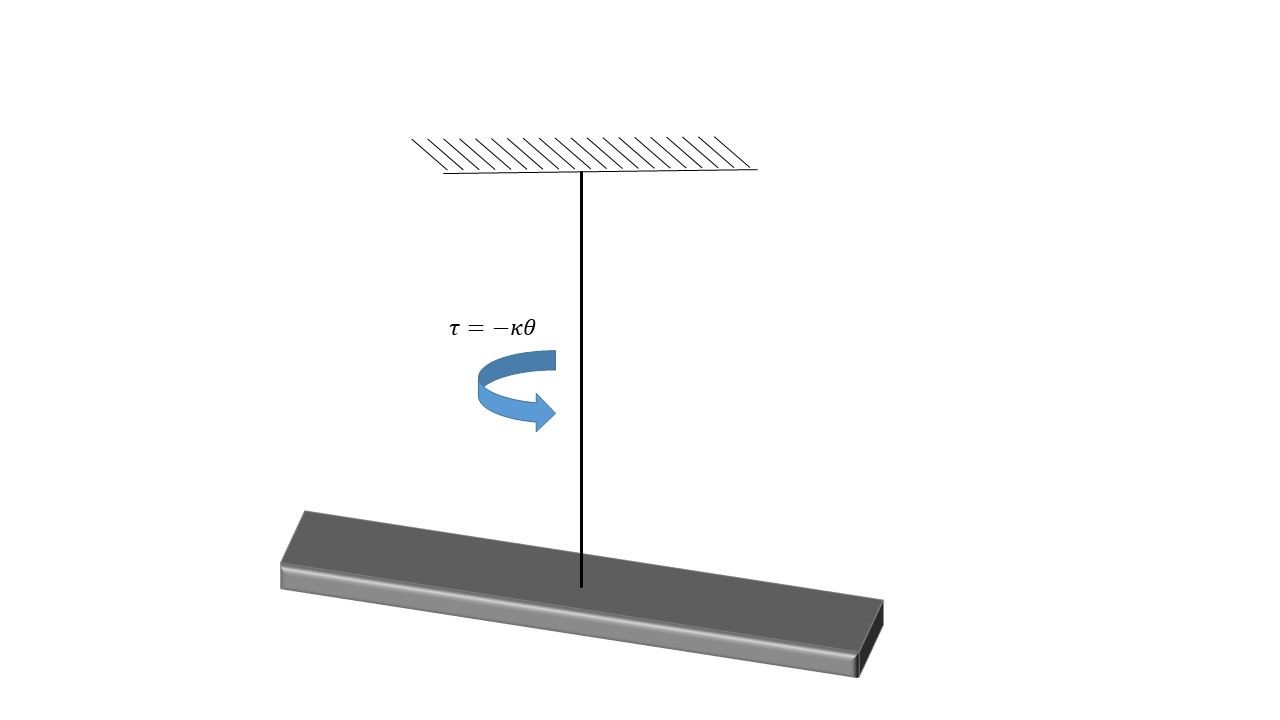
\includegraphics[width=0.4\textwidth,keepaspectratio]{torsion_pendulum_powerpoint.jpg}
    \end{center}
	\begin{itemize}

		\item Torsional pendulum is an oscillator made of a mass hung by a string. 
		\pause
		\item When the mass is displaced from equilibrium angle, there is a linear restoring torque $\tau = -\kappa\cdot\theta$.
		\pause
		\item The torsional pendulum is an angular harmonic oscillator.
		\pause
		\item The restoring torque causes sinusoidal oscillations around the equilibrium angle: $\theta(t) = \theta_{max}cos(\omega_0 t )$
		
	\end{itemize}
\end{frame}


% frame 2
\begin{frame}{Damped oscillator}
	
	\begin{itemize}	
		\item The pendulum is a damped oscillator if there is a damping torque opposite to the angular velocity $\tau = -b\dot{\theta}$.
		\pause
		\item The damped motion is given by $\ddot{\theta} + 2\xi\omega_0\dot{\theta} + \omega_0^2\theta = 0$.
		\pause
		\item The damping ratio, $\xi$, determines the oscillator's motion: underdamped, critically damped or overdamped.
	\end{itemize}
	\begin{center}		
		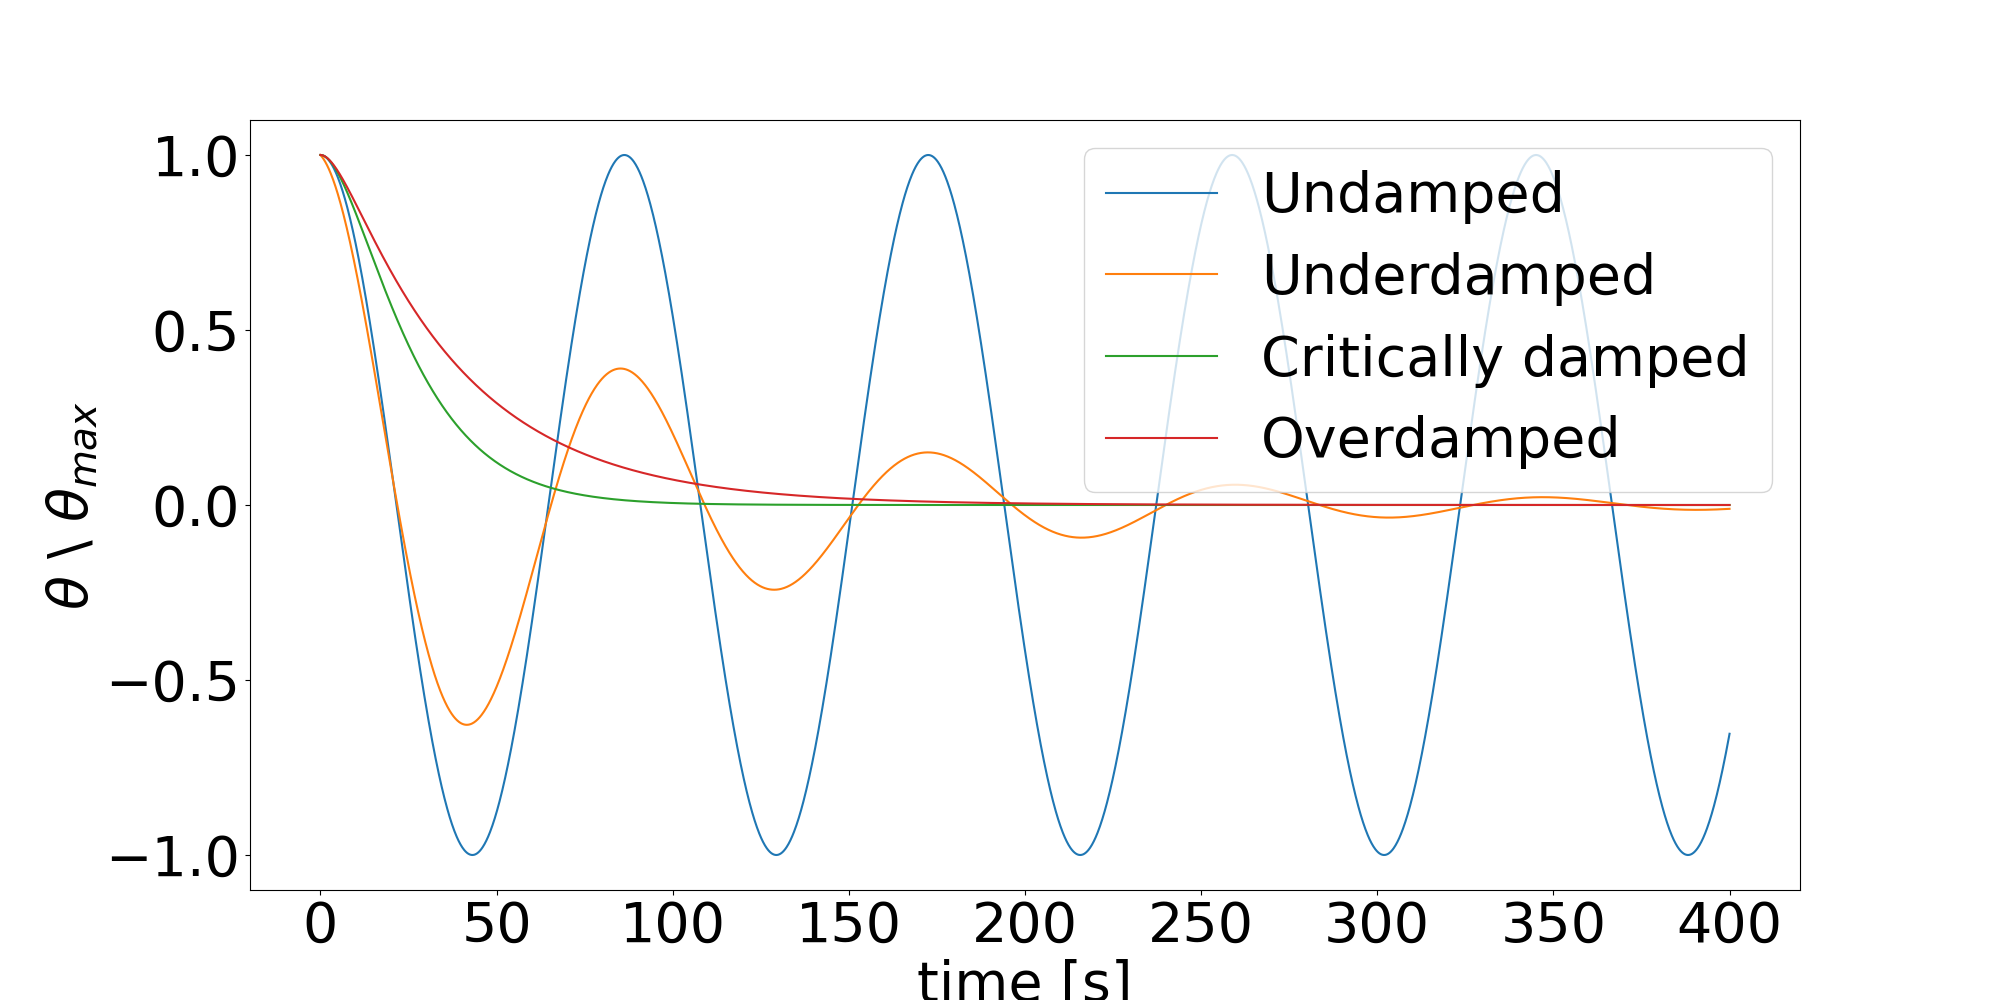
\includegraphics[width=0.5\textwidth,keepaspectratio]{damp.png}
    \end{center}
	
\end{frame}

% frame 3
\begin{frame}{Damped oscillator}
	
	\begin{itemize}
		\item Undamped; harmonic oscillations without decay.
		\pause
		\item Underdamped; oscillations amplitude decreases in time while oscillating with a lower frequency.
		\pause
		\item Critically damped; oscillator cannot oscillate and decays exponentially to equilibrium position.
		\pause
		\item Overdamped; oscillator with exponential decay and longer damping time than critical damping. 
		\pause
		\item The pendulum is a driven oscillator if there is also a time-dependent torque $\tau(t)$.
	\end{itemize}
\end{frame}
\subsection{Gravity measurement}
% frame 1
\begin{frame}{Gravitational field}
	
	\begin{itemize}
		\item Newton's law of universal gravitation: $\overrightarrow{F}(r) = \frac{GMm}{r^2}\hat{r}$
		\pause
		\item Since the gravitational constant is small, the force is weak.
		\pause
		\item The gravitational field of mass $M$ is consisted of vectors pointing directly towards the mass: $\overrightarrow{g}(r) = \frac{\overrightarrow{F}(r)}{m} = \frac{GM}{r^2}\hat{r}$ 
		\end{itemize}
\end{frame}
% frame 2
\begin{frame}{Cavendish apparatus}
\framesubtitle{Setup}
	\begin{center}		
		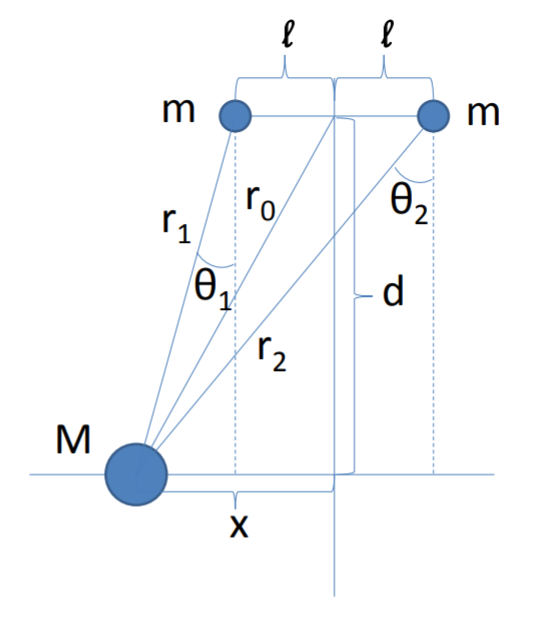
\includegraphics[width=0.25\textwidth,keepaspectratio]{Cavendish apparatus.PNG}
    \end{center}
	\begin{itemize}
		\item The Cavendish apparatus measures the gravitational force of test mass $M$ using a torsional pendulum.
		\pause
		\item The pendulum can be assumed to consist of two masses $m$ connected by a rigid, massless thin rod, with length of $2l$, and a pivot point at distance $l$ from each mass.
		\pause
		\item The mass $M$, located at distance $r_0$ from the pivot point attracts the two masses and creates gravitational torques.
	\end{itemize}
\end{frame}
% frame 3
\begin{frame}{Cavendish apparatus}
\framesubtitle{Measurement}
	\begin{center}		
		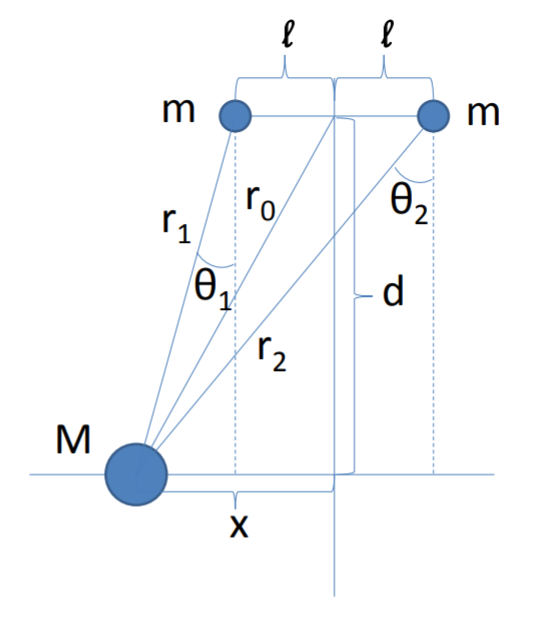
\includegraphics[width=0.25\textwidth,keepaspectratio]{Cavendish apparatus.PNG}
    \end{center}
	\begin{itemize}
		\item The net gravitational torque is the sum of the two torques, one from each mass: $\tau_g = l \cdot F(r_1) \cdot cos\theta_1 - l \cdot F(r_2) \cdot cos\theta_2$
		\pause
		\item If $l<<d,x,r_0$ the net torque can be approximated to: $\tau_g =  \frac{6l^2GmMxd} {r_0^5} = \frac{6l^2GmM sin\theta cos\theta}{r_0^3}$
		\item Where $\theta$ is the tilt angle of the torsional pendulum and approximately $\theta_1 \approx \theta_2 = \theta$.
	\end{itemize}
\end{frame}
% frame 4
\begin{frame}{Cavendish apparatus}
	\framesubtitle{Approximation}
	\begin{center}		
		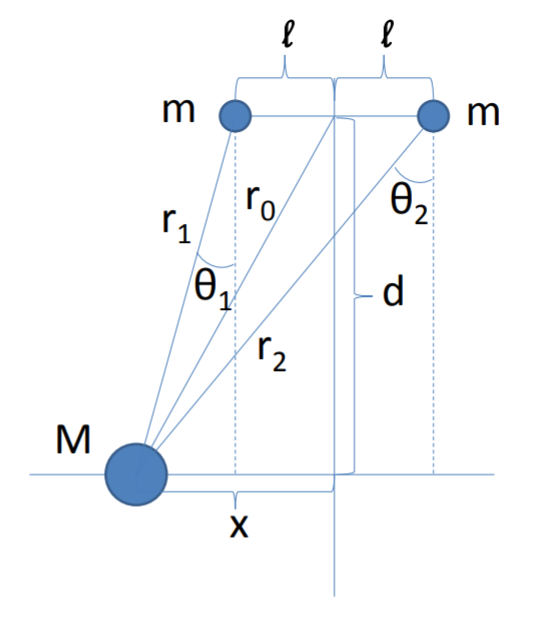
\includegraphics[width=0.25\textwidth,keepaspectratio]{Cavendish apparatus.PNG}
    \end{center}
	\begin{itemize}
		\item The net gravitational torque: $\tau_g =  l d GmM(\frac{1}{r_1^3} - \frac{1}{r_2^3})$.
		\item Defining the function: $h(l) = \frac{1}{(d^2 +(x-l)^2)^{3/2}}$.
		\item If $l<<d,x,r_0$ one can approximate: $h(l)-h(-l)\approx h'(0)\cdot 2l = \frac{6lx}{r_0^5}$.
		\item the net torque is proportional to the difference: $\tau_g = l d GmM[h(l)-h(-l)]\approx \frac{6l^2GmMxd} {r_0^5}$.
	\end{itemize}
\end{frame}
% frame 5
\begin{frame}{Simple harmonic oscillator}
	\framesubtitle{Gravitational measurement}
	\begin{center}		
		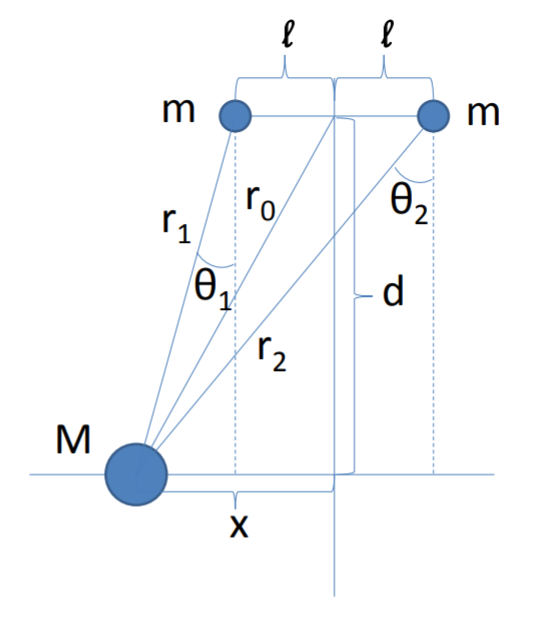
\includegraphics[width=0.25\textwidth,keepaspectratio]{Cavendish apparatus.PNG}
    \end{center}
	\begin{itemize}
		\item Assuming no damping force (simple harmonic motion).
		\pause
		\item when test mass $M$ is introduced, there are the gravitational net torque and an inverse torsional restoring torque.
		\pause
		\item At equilibrium, the torques cancel each other out $\tau_g =  \kappa\theta$.
		\pause
		\item The average equilibrium angle: $\overline{\theta} = \frac{\tau_g}{\kappa} \approx \frac{3GT^2cos\theta sin\theta}{4\pi^2 } \cdot \frac{M}{r_0^3}$.
		
	\end{itemize}
\end{frame}
% frame 6
\begin{frame}{Gravity sensing}
	
	
	\begin{itemize}
		
		\item The sensor's tilt angle is measured at each frequency, measuring the energy spectral density $[\frac{rad}{\sqrt{Hz}}]$ of the sensor.
		\pause
		\item By integrating over long periods, measurement noises are reduced. The signal to noise ratio (SNR) is the limiting factor for the sensitivity of a measuring system.
		\pause
		\item At higher frequencies the integration is faster, reducing more noises and having higher SNR.
		\pause
		\item The SNR dependency on frequency is a significant challenge while designing gravimetric sensors for low frequencies.

	\end{itemize}
\end{frame}


\subsection{Environment affects}
\begin{frame}{Ideal gas}
	\begin{itemize}
		\item An ideal gas is a theoretical gas composed of gas particles without inter-particle interactions: $PV =  N k_B T $.
		\item The torsional pendulum interacts with an ideal gas environment, causing pressure-dependent noise and friction.
		\pause
		\item At higher pressures (gas with turbulent flow), drag force is $F = -b(P)\cdot v^2 $.
		\item At lower pressures (gas with laminar flow), the drag force is given by Stokes' law: $F_{drag} =  -b(P)\cdot v$.
		
	\end{itemize}
\end{frame}

\begin{frame}{Environmental noises}
	\begin{itemize}
		
		\item Brownian motion causes random particles' fluctuations at thermal equilibrium in a given temperature. The kinetic energy of the gas particles: $ N<E_k> = \frac{3}{2} PV$.
		\item Acoustic waves are adiabatic waves propagating through a material. The average power at room temperature $p  \approx 1\cdot10^{-22}AP^2$.
		\item Heat flow is the exchange of thermal energy between physical systems. The net power is: $p= A P c_v \Delta T \sqrt{\frac{M}{RT}} $.
		\pause
		\item The net absorbed power due to environment black body radiation is $p= A \sigma\epsilon[ T^4- T_0^4]$.
		
	\end{itemize}
\end{frame}

\subsection{The damping process}

\begin{frame}{Proportional–integral–derivative (PID) controller}
	\begin{center}		
		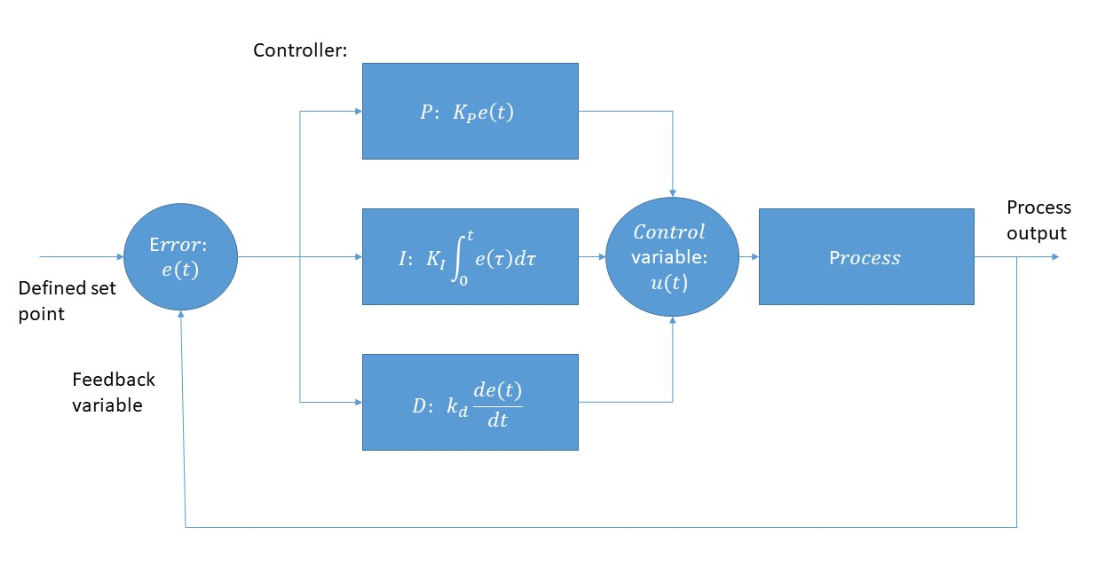
\includegraphics[width=0.6\textwidth,keepaspectratio]{pid_diagram_powerpoint.jpg}
    \end{center}
	\begin{itemize}	
		\item PID controller is a feedback based control system, for time continuous control of a process.
		\item The PID continuously calculates error value $e(t)$ from the defined set point. 
		\pause
		\item The feedback applies an external correction to the process.
		\item The control is based on a proportional, integral and derivative response to the error (P-I-D).
	\end{itemize}
\end{frame}

\begin{frame}{Proportional–integral–derivative (PID) controller}
	\begin{center}		
		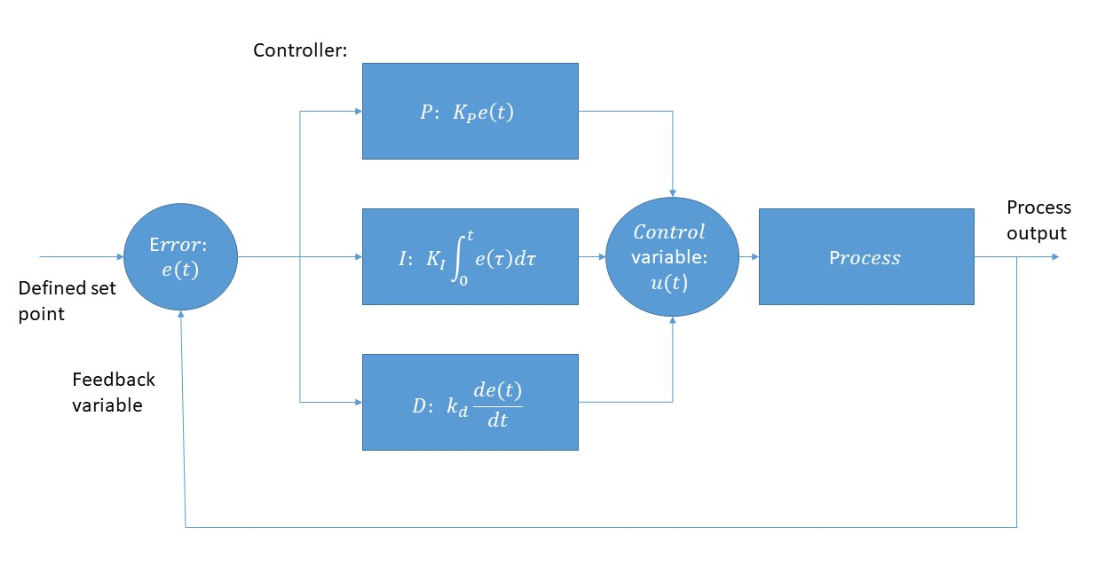
\includegraphics[width=0.6\textwidth,keepaspectratio]{pid_diagram_powerpoint.jpg}
    \end{center}
	\begin{itemize}	
		\item Each response is assigned to a tunable gain. the PID output is a weighted sum of the response terms.
		\item $u(t) = K_P e(t)+K_I\int_{0}^{t}e(\tau)d\tau+K_D\frac{de(t)}{dt}$
		\pause
		\item Over time the PID controller attempts to minimize the error by adjusting the output.
	\end{itemize}
\end{frame}
\begin{frame}{Radiation-pressure}
	\begin{itemize}
		
		\item The pressure of a light beam on the surface due to momentum exchange with the electromagnetic field.
		\pause
		\item The radiation-pressure force depends on the surface angle relative to the field propagation direction, the surface reflectance and absorbance, and the hitting light power.
		\pause
		\item When the light field direction is perpendicular to a reflective surface the radiation force is: $F  \approx\frac{2\eta\Theta_{source}}{{c}} $.
		\pause
		\item The apparatus PID external correction is made by generating Radiation-pressure force.
	\end{itemize}
\end{frame}
\section{Thesis aims}
\begin{frame}{Cavendish experiment}
	\begin{itemize}
		
		\item The Cavendish experiment, is constructed using a torsional pendulum with a front mirror. Optical measurement of angle displacement is made with a quadrant detector.
		\item The measurement sensitivity is limited by noise. The technical noise is greater than the fundamental noise. Reducing the noise enables higher sensitivity.
		\pause
		\item The measurement is fundamentally limited by quantum uncertainty and the measurement system shot noise. 
		
	\end{itemize}
\end{frame}

\begin{frame}{Damping process}
	\begin{itemize}
		
		\item Assuming above basic energy level the quantum uncertainty due to thermal energy is temperature dependent: $\delta\theta = \sqrt{\frac{k_B T}{\kappa}} \approx 4\cdot 10^{-8} [rad]$.
		\item The shot noise limit is: $\delta\theta \approx 10^{-14} [\frac{rad}{Hz}] $.
		\pause
		\item The torsional pendulum is placed inside a vacuum chamber reducing pressure-dependent noise. 
		\item The noise reduction allows active damping of the remaining noises using a PID controller. 
		\item With PID tuned correctly the damped pendulum is at critical damping and oscillations become smaller.

		
	\end{itemize}
\end{frame}

\begin{frame}{Gravitational measurement}
	\begin{itemize}
		
		
		\item When amplitude is smaller than the fundamental limit, the PID is effectively reducing the pendulum's temperature. 
		\pause
		\item Introducing a new mass adds a constant new torque to the system $\tau_g$. The PID error changes to $e(t) = \delta\theta(t) + \theta_g(t)$.
		\item The PID is compensating for the new error, the response becomes mainly an inverse torque: $\tau_{PID}(t) \approx K_P\theta_g(t)$. 
		\item When integrating over short periods the gravitational angle is constant: $\overline{\theta}_g =  \frac{\int \tau_{PID}(t) dt}{ K_P \Delta t} $
		\pause
		\item The measurement system allows fast response (short integration time) with increased measurement sensitivity.
		
	\end{itemize}
\end{frame}

\section{Methods and results}

\subsection[Basic Problem]{The basic problem that we have studed}

\begin{frame}{Slide Title \#1}
	\framesubtitle{Slide subtitle \#1}
	\begin{itemize}
		\item Use the \texttt{itemize} environment frequently.
		\pause
		\item Use short sentences and phrases.
		\pause
		\item In this presentation we use the \textbackslash{}\texttt{pause} macro.
	\end{itemize}
\end{frame}

\begin{frame}{Slide Title \#2}
	\begin{itemize}
		\item <1->You can define the order of appearance.
		\item <3->Like here.
		\item <2->This is the second item to appear.
	\end{itemize}
\end{frame}

\begin{frame}{Slide Title \#3}
	\begin{block}
		<1->{}
		\begin{itemize}
			\item Group without title.
			\item Appears for all slides.
		\end{itemize}
	\end{block}
	\begin{exampleblock}
		<2->{Group title}
		\begin{itemize}
			\item $e^{i\pi}=-1$.
			\item $e^{i\pi/2}=i$.
		\end{itemize}
	\end{exampleblock}
\end{frame}

%%
\subsection{Previous work}

\begin{frame}{Slide Title \#4}
	\begin{example}
		<1->First example. 
	\end{example}
	\begin{example}
		<2->Second example.
	\end{example}
\end{frame}

\begin{frame}{Slide Title \#5}
	\begin{center}
		Table example \\[12pt]
		\begin{tabular}{c||c|c|c|}
			& \textbf{col 1} & \textbf{col  2} & \textbf{col 3} \\
			\hline
			\hline
			\textbf{row 1} & 11 & 12 & 13 \\
			\hline
			\textbf{row 2} & 21 & 22 & 23 \\
		\end{tabular}
    \end{center}
\end{frame}

\begin{frame}{Slide Title \#6}
	\begin{center}
		Figure example \\[12pt]
		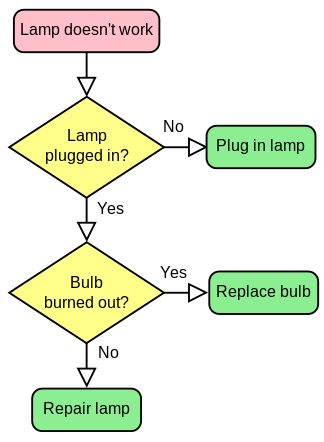
\includegraphics[width=0.35\textwidth,keepaspectratio]{LampFlowchart.png}
		\\
		\footnotesize(source: \textlatin{Wikipedia})
    \end{center}
\end{frame}

\begin{frame}{Slide Title \#7}
	\centering
	Math examples \\[12pt]
	\begin{equation}
        	B'=-\nabla \times E
	\end{equation}
	\begin{equation*}
        	E'=\nabla \times B - 4\pi j
	\end{equation*}
\end{frame}

%%%%
\section{Results / contribution}

%%
\subsection{Main results}

\begin{frame}{Summary}
   	\begin{alertblock}{Attention}
   		\textlatin{This is an important alert}
   	\end{alertblock}
\end{frame}

%
\subsection{Subsection title}

\begin{frame}{Summary}
	\begin{itemize}
		\item The \textcolor{red}{first main message} of our talk.
		\item The \textcolor{red}{second main message} of our talk.
		\item Maybe a \textcolor{red}{third message}, but ... no more.
	\end{itemize}
	\vskip0pt plus.5fill
	\begin{itemize}
		\item Conclusion.
	\end{itemize}
	\begin{itemize}
		\item Future work.
		\item Discussion.
	\end{itemize}
\end{frame}

\begin{frame}{References}
	\begin{thebibliography}{2}
		\beamertemplatebookbibitems
		\bibitem{Author1990}A.\ Author. \newblock\emph{Handbook of Everything}.\newblock
\textlatin{Some Press, \oldstylenums{1990}}.

		\beamertemplatearticlebibitems
		\bibitem{Someone2002}B.\ Author.\newblock On this and that\emph{.}
\newblock\emph{Journal on This and That}. 
\oldstylenums{2}(\oldstylenums{1}):\oldstylenums{50}--\oldstylenums{100}, 
\oldstylenums{2000}.
	\end{thebibliography}
\end{frame}

%%
\end{document}